% !Mode:: "TeX:UTF-8"
%% 请使用 XeLaTeX 编译本文.
\documentclass{WHUMaster}   % 选项 forprint: 交付打印时, 建议加上此选项, 以消除彩色链接文字, 避免彩色字迹打印偏淡.
                                              % 选项 forlib: 提交给图书馆的电子版, 需要加上选项 forlib, 以消除空白页和彩色链接.
                                              % 选项 smd: Specialist Master's Degree, 产生专业硕士学位论文封面、页眉.
                                              
%%%=== 参考文献=== %%%
\bibliographystyle{abbrv}        % 参考文献样式,  plain,unsrt,alpha,abbrv 等等
%%%%%%%%%%%%%%%%%%%%%%%%%%%%%%%%%%%%%%%%%%%%%%%%%%%%
\usepackage{booktabs}
\usepackage{multirow}
\usepackage{array}
\usepackage{xpatch}
\makeatletter
\xpatchcmd{\chapter}
{\if@openright\cleardoublepage\else\clearpage\fi}{\par\relax}
{}{}
\makeatother
\usepackage{blindtext}
\begin{document}
%%%%%%%-------------------------------------------------

\fenleihao{自1602}  % 分类号:《中国图书资料分类法》的类号. 必填. 要根据自己的学科方向填写!!
\miji{1802160115}                % 密级
\UDC{}               %《国际十进制分类法UDC》的类号. 选填.
\bianhao{10486}  % 学校编号, 10486是武汉大学的编号. 不用改动.

\title{基于simulink的三容水箱液位控制仿真}
\Etitle{A \LaTeX~Thesis Template for Wuhan University} % 英文题目
\author{李泽中}
\StudentNumber{1802160115}   % 学号
\Eauthor{HUANG Zhenghua}            %作者英文名
\Csupervisor{薄翠梅\quad 教授}        %指导教师中文名、职称
\Esupervisor{Prof.~HU Bao Qing}     %指导教师英文名、职称
\Cmajor{自动化}                          % 专业中文名[ SMD:专业类别(领域)]
\Emajor{Computational Mathematics}% 专业英文名[ SMD:专业类别(领域)]
\Cspeciality{智能计算}                     % 研究方向
\Especiality{Intelligent Computing}   % 研究方向
\Schoolname{School of Mathematics and Statistics} %学院英文名. 不确定的话, 请看一下自己学院的网页上是怎么写的. 别搞错了!
\date{二〇一九年三月}                % 硕士类只写年月. 要注意和英文日期一致!!
\Edate{May, 2016}                   % 英文封面日期

%-----------------------------------------------------------------------------
\pdfbookmark[0]{封面}{title}         % 封面页加到 pdf 书签
\maketitle
%-----------------------------------------------------------------------------
% !Mode:: "TeX:UTF-8"

%%% 此部分包含: (1) 英文封面 (无需改动) ; (2) 郑重声明 (无需改动).

%%%%%%%%%%%%%%%%%%%%%%%%%%%%%
%%% -------------  英文封面 (无需改动)-------------   %%%
%%%%%%%%%%%%%%%%%%%%%%%%%%%%%
%\thispagestyle{empty}
%\renewcommand{\baselinestretch}{1.5}  %下文的行距
%\vspace*{0.5cm}

%\begin{center}{\zihao{2} \the\Etitle \par}\end{center}

%\vfill

%\begin{center}
%\zihao{4}
%\begin{tabular}{ r l }
% Candidate:      &  {\sc \the\Eauthor}      \\
% Student Number: & {\the\StudentNumber} \\
% Supervisor:     &  {\sc \the\Esupervisor}   \\
% Major:          & \the\Emajor  \\
%\ifsmd \else Speciality:     & \the\Especiality \fi
%\end{tabular}

%\vspace*{2cm}
%\begin{center}
%  \iflib % 向图书馆提交电子文档, 使用黑白校徽.
%  
\includegraphics[height=4cm]{whu.eps}       %%  黑白的. 很小, 只有 10k.
%  \else
%     \ifprint % 文档打印, 使用黑白校徽.
%  
\includegraphics[height=4cm]{whu.eps}       %%  黑白的.
%  \else
%  
\includegraphics[height=4cm]{whulogo.eps} %%  彩色的.
%  \fi
%  \fi
%\end{center}


%\zihao{-2}
%\the\Schoolname\\
%{\sc Wuhan University}

%\vspace*{1.0cm}

%\the\Edate

%\end{center}
%%%%%%%--判断是否需要空白页-----------------------------
%  \iflib
%  \else
  %\newpage
%  \thispagestyle{empty}
%  \cleardoublepage
%  \fi
%%%%%%%-------------------------------------------------
%%%--- 加入``郑重声明'' --- %%%%%%%%%%%%%%%%%
%{\pagestyle{empty}
%\newpage
%\vspace*{20pt}
%\begin{center}{\ziju{0.8}\zihao{-2}\heiti 论文原创性声明}\end{center}
%\par\vspace*{30pt}
%\renewcommand{\baselinestretch}{2}
%{\zihao{4} \songti %


%本人郑重声明: 所呈交的学位论文, 是本人在导师指导下, 独立进行研究工作所取得的研究成果.
%除文中已经标明引用的内容外, 本论文不包含任何其他个人或集体已经发表或撰写过的研究成果.
%对本文的研究做出贡献的个人和集体, 均已在文中以明确方式标明. 本声明的法律结果由本人承担.


%\vskip2cm

%\hspace*{4cm}学位论文作者(签名): \hspace{4cm} \hfill \\[1cm]
%\hspace*{10cm}年 \hfill  月 \hfill 日\hspace{1cm}\hfill\par}

%%%%%%%--判断是否需要空白页-----------------------------
%  \iflib
%  \else
%  \newpage
%  \cleardoublepage
%  \fi
%%%%%%%-------------------------------------------------
%}
%\renewcommand{\baselinestretch}{1.6}
%\small\normalsize




    % 加入英文封面
\frontmatter
\pagenumbering{Roman}               % 正文之前的页码用大写罗马字母编号.

\cleardoublepage
\newpage  \pagestyle{fancy} \fancyfancy
%------------------------------------------------------------------------------
% !Mode:: "TeX:UTF-8"

%%% 说明: 此部分需要自己填写的内容:  (1) 中文摘要及关键词 (2) 英文摘要及关键词

%%%%%%%%%%%%%%%%%%%%%%%
%%% ------------ 中文摘要 ---------------%%%
%%%%%%%%%%%%%%%%%%%%%%%
\begin{cnabstract}
本文主要介绍和讨论了武汉大学硕士毕业论文的~\LaTeX~模板.
指明了编译方法, 强调了公式排版的一些细节问题, 也指出了一些常见的排版错误.



\end{cnabstract}
\vspace{1em}\par\vfill

%%%--------- 关键词 -------- %%%
\cnkeywords{毕业论文, \LaTeX{}, 模板, XeLaTeX }

%%%%%%%%%%%%%%%%%%%%%%%


%%%%%%%%%%%%%%%%%%%%%%%
%%% ------------ 英文摘要 ---------------%%%
%%%%%%%%%%%%%%%%%%%%%%%

%\begin{enabstract}
%This thesis is a study on the theory of \dots.




%\end{enabstract}
%\vspace{1em}\par\vfill

%%%------ 英文关键词 ------- %%%
%\enkeywords{\LaTeX{}, XeLaTeX, \dots}


      % 加入中英文摘要.
%---把目录加入到书签---%%%%%%%%%%%%%%
\pdfbookmark[0]{目录}{toc}%%%%%%%%%%%%

\tableofcontents

%------------------------------------------------------------------------------
\mainmatter %% 以下是正文
\baselineskip=20pt  % 正文行距为 20 磅
%%%%%%%%%%%%%%%%%%%%%%%%%%%%%%%%%%%%

\chapter{基于simulink的PID半经验法参数整定}
\section{半经验法概述}
所谓PID参数的整定,就是通过选择合适的比例系数$K_p$ 、积分时间常数$T_i$和微分时间$T_d$,使PID控制器能够将系统调节到最佳的运行状态。PID参数的整定方法主要有:经验整定法,半经验法和理论计算法。其中,半经验法采用单纯P作用先行搜索,获得所需衰减的响应曲线,然后根据相应参数,利用半经验公式计算出PID控制器的参数。工程整定的半经验法不需要获得调节对象的准确动态特性,直接在闭合的调节回路中进行整定,方法简单、 计算方便、容易掌握,适合在工程实际中应用。

图\ref{fig1}是基于simulink的PID半经验法整定实例,其中$G_p$模块的传递函数为:$\frac{3.5}{10s^2+7s+1}$.在进行半经验法PID参数整定之前,我们做了以下两点准备工作:
\begin{itemize}
	\item 考虑到matlab的绘图函数拥有比simulink中scope更强的绘图能力,我们在系统中添加了“simout”模块,用以将系统的阶跃响应数据以时间序列的形式传输至matlab中的workspace,方便曲线绘制
	\item 为了使响应曲线更加完整,将仿真时间调至“100s”
\end{itemize}
\begin{figure}[h]
	\small
	\centering
	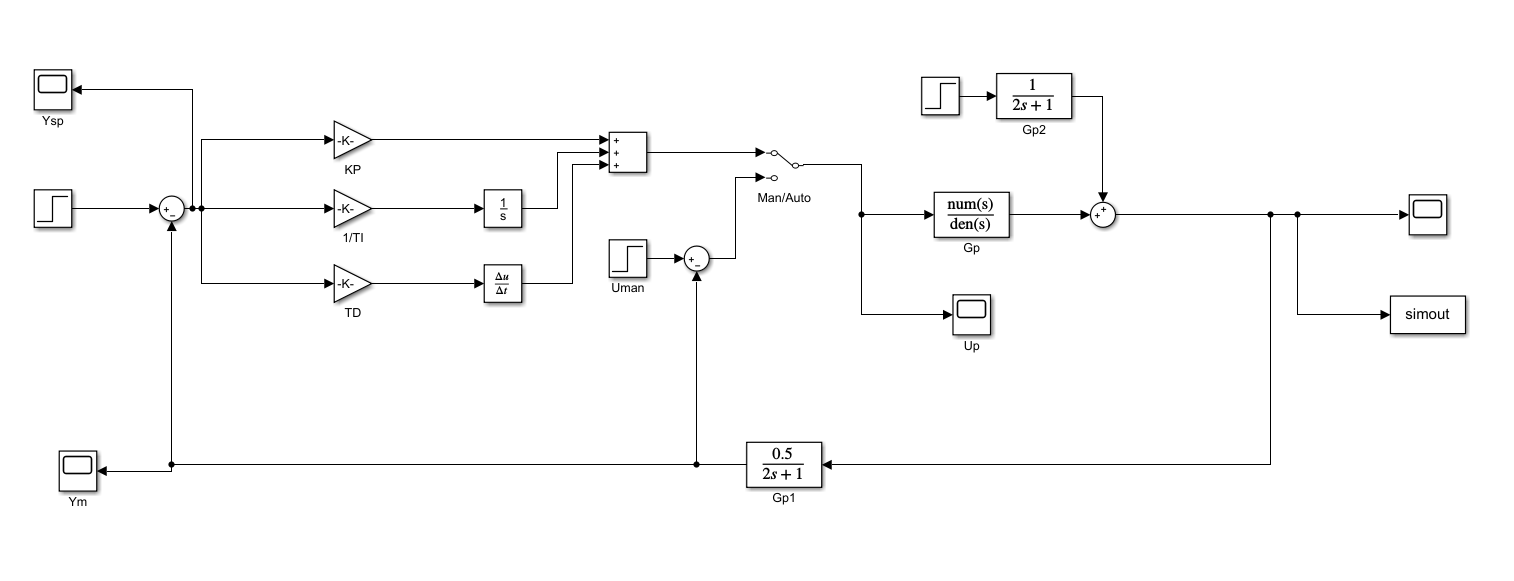
\includegraphics[width=12cm]{pid4simulink2.png}
	\caption{基于simulink的PID半经验法参数整定实例} \label{fig1}
\end{figure}

将模块$K_p$的值调至1,模块$\frac{1}{T_i}$和$T_d$调至0,进行仿真,并用matlab的plot函数绘制出未加PID的系统的响应曲线。

\begin{figure}[h]
	\small
	\centering
	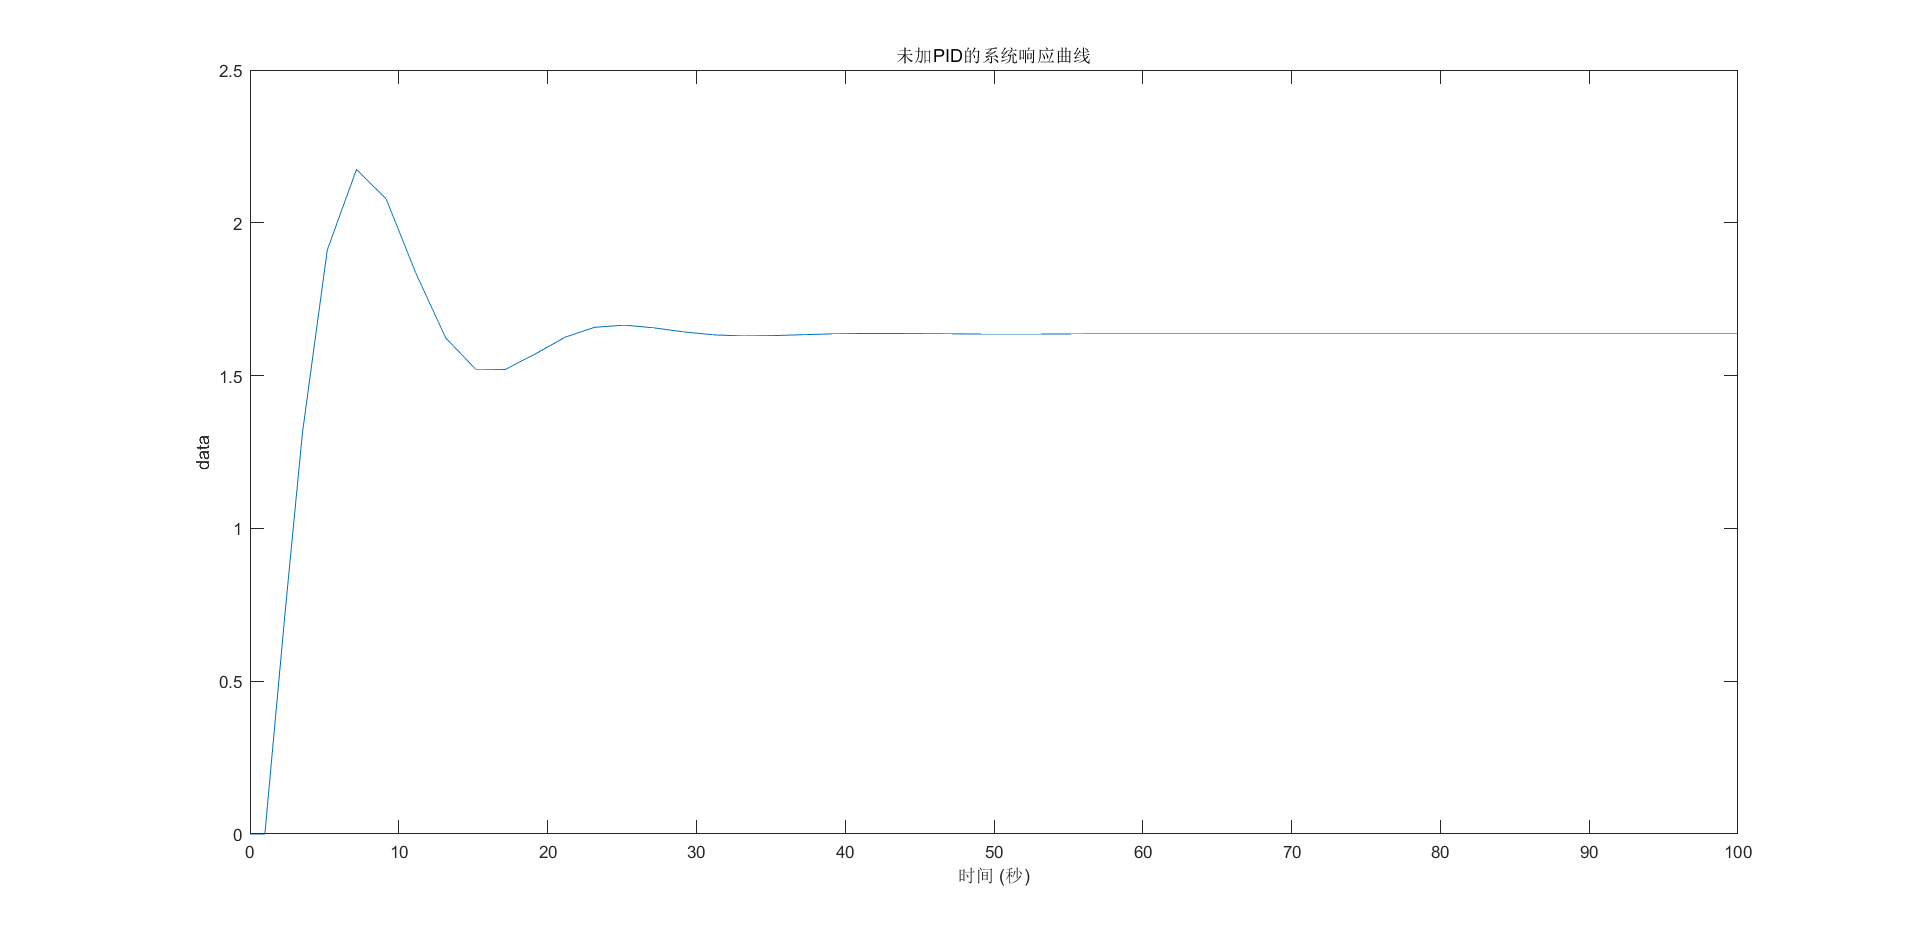
\includegraphics[width=12cm]{weijia.png}
	\caption{未加PID响应曲线} \label{fig2}
\end{figure}

图\ref{fig2}显示了未加PID控制器前的响应曲线。从图中可以看出,系统能够稳定运行,但存在稳态误差。下文将分别选用PI和PID控制器,并采用临界比例度法和衰减曲线法两种半经验方法进行参数整定,并对整定结果进行分析和改进,希望通过PID校正,能够使系统消除稳态误差,并且改善其快速性。
\section{临界比例度法}
临界比例度法又称Ziegler-Nichols整定法。调整方法是:先调整比例度,使过渡过程为等辐震荡,这时的比例度为临界比例度$\delta _k$,振荡周期为临界振荡周期$T_k$,可按表\ref{tab1}整定控制器参数。

\begin{table}[htbp]
	\centering
	\caption{临界比例度法整定控制器参数}
	\begin{tabular}{cccccccc}
		\toprule
		\multicolumn{2}{c}{\multirow{2}[4]{*}{控制作用}} & \multicolumn{6}{c}{临界比例度法} \\
		\cmidrule{3-8}    \multicolumn{2}{c}{} & \multicolumn{2}{c}{$\delta$/\%} & \multicolumn{2}{c}{$T_i$} & \multicolumn{2}{c}{$T_d$} \\
		\midrule
		\multicolumn{2}{c}{P} & \multicolumn{2}{c}{2$\delta _k$} & \multicolumn{2}{c}{} & \multicolumn{2}{c}{} \\
		\midrule
		\multicolumn{2}{c}{PI} & \multicolumn{2}{c}{2.2$\delta _k$} & \multicolumn{2}{c}{0.85$T_k$} & \multicolumn{2}{c}{} \\
		\midrule
		\multicolumn{2}{c}{PID} & \multicolumn{2}{c}{1.7$\delta _k$} & \multicolumn{2}{c}{0.50$T_k$} & \multicolumn{2}{c}{0.125$T_k$} \\
		\bottomrule
	\end{tabular}%
	\label{tab1}%
\end{table}%

具体整定过程如下:
\begin{itemize}
		\item 在$K_p$模块中将比例系数$K_p$设置一个一个较大的初值100并运行(注意:在实际场合进行PID控制器参数整定时绝对不能将比例系数$K_p$预设一个较大的值,在仿真过程中采用本方法可以迅速找到合适的$K_p$),在matlab中用plot函数绘制本次响应曲线,曲线呈发散震荡形式 
		\item 采用数学中的二分法进行搜索,即:将比例系数$K_p$逐次减半($K_p$=50,25,12.5,6.25···),直到曲线等幅振荡
		\item 记录此时的比例系数$K_p$=5.6 和临界振荡周期$T_k$=9.3593,根据$K_p$=5.6求得临界比例度$\delta _k=\frac{1}{K_p}\times \text{100\%}=\text{17.85\%}$
		\item 根据表\ref{tab1}记录得到控制作用为PID时$K_p=\frac{1}{1.7\times \text{17.85\%}}=3.29544$,$\frac{1}{T_i}=\frac{1}{0.5\times 9.3593}=0.2137$,$T_d=0.125\times 9.3593=1.16991$,控制作用为PI时$K_p=\frac{1}{2.2\times \text{17.85\%}}=2.5454$,$\frac{1}{T_i}=\frac{1}{0.85\times 9.3593}=0.1257$
\end{itemize}
图\ref{fig3}显示了采用临界比例度法分别整定PID和PI控制作用参数后的系统响应曲线,从图中可以明显看出:得益于微分作用的加入,PID曲线的上升时间略短,快速性优于PI控制;但两者的超调量达到了稳态值的75\%,并且最终达到稳态的时间过长,大约在70s左右。临界比例度法的参数整定结果虽然可以令系统消除稳态误差,但快速性和超调量两方面仍有待提高。
\begin{figure}[h]
	\small
	\centering
	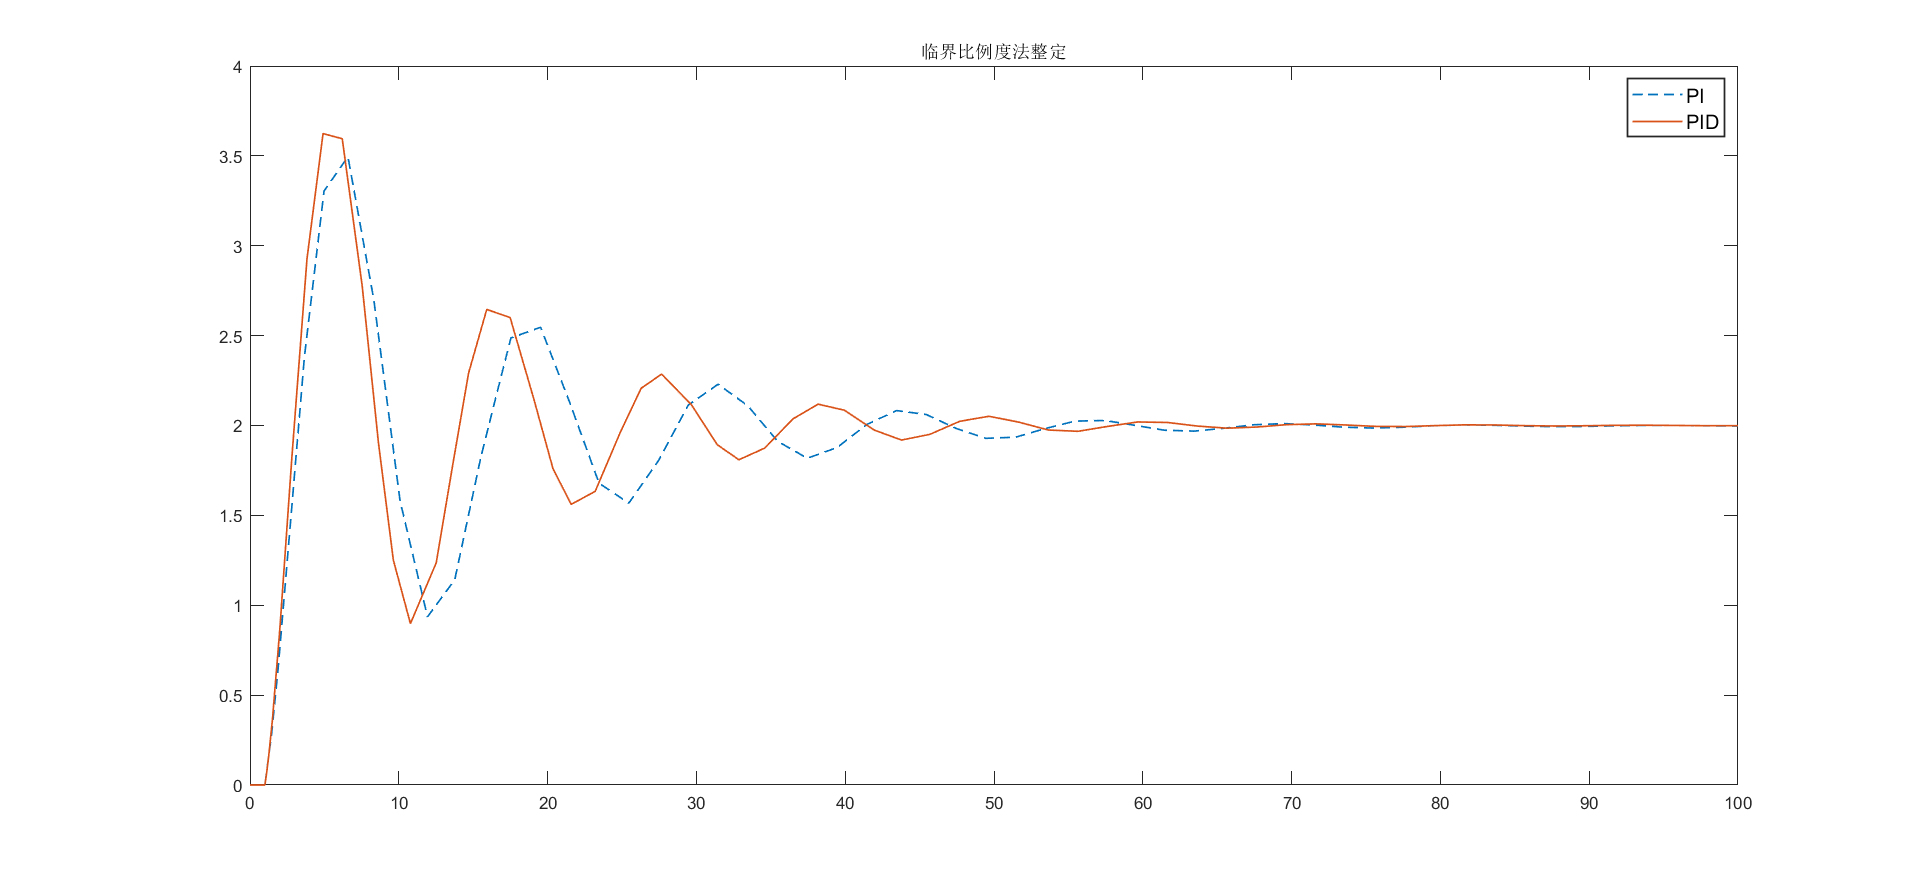
\includegraphics[width=12cm]{linjie.png}
	\caption{临界比例度法整定结果} \label{fig3}
\end{figure}

\section{衰减曲线法}
衰减曲线法和临界比例度法具有类似的调整方式,即通过调整比例系数$K_p$,使控制系统过渡过程响应曲线的衰减比为10:1(随动控制系统),得到上升时间$t_r$或4:1(定制控制系统),得到系统的振荡周期$T_p$,此时比例度为$\delta _s$,按表\ref{tab1}整定P,PI或PID控制器的参数。

\begin{table}[htbp]
	\centering
	\caption{衰减曲线法整定控制器参数}
	\begin{tabular}{cc|cc|cc|cc}
		\toprule
		\multicolumn{2}{c|}{\multirow{2}[4]{*}{控制作用}} & \multicolumn{6}{c}{衰减曲线法} \\
		\cmidrule{3-8}    \multicolumn{2}{c|}{} & \multicolumn{2}{c|}{$\delta$/\%} & \multicolumn{2}{c|}{$T_i$} & \multicolumn{2}{c}{$T_d$} \\
		\midrule
		\multicolumn{2}{c|}{P} & \multicolumn{2}{c|}{$\delta _s$} & \multicolumn{2}{c|}{} & \multicolumn{2}{c}{} \\
		\multicolumn{2}{c|}{PI} & \multicolumn{2}{c|}{1.2$\delta _s$} & \multicolumn{2}{c|}{2$t_r$或0.5$T_p$} & \multicolumn{2}{c}{} \\
		\multicolumn{2}{c|}{PID} & \multicolumn{2}{c|}{0.8$\delta _s$} & \multicolumn{2}{c|}{1.2$t_r$或$T_p$} & \multicolumn{2}{c}{0.4$t_r$或0.1$T_p$} \\
		\bottomrule
	\end{tabular}%
	\label{tab2}%
\end{table}%
具体整定过程如下:
\begin{itemize}
	
\item 对于同一系统,我们通过临界比例度法已经得到可以使产生等幅振荡的比例系数$K_p$=5.6,此时等幅振荡的曲线衰减比为1:1(衰减比定义为两个相邻同方向幅值之比,在本例中视为第一个波峰峰值与稳态值之差同第二个波峰峰值与稳态值之差的比值)。
\item 继续运用二分法,小范围调整比例系数$K_p$的值,得到产生衰减比4:1的$K_p$=2.255,记录此时的震荡周期$T_p$=13.3309
\item 根据表\ref{tab2}记录得到控制作用为PID时$K_p=\frac{1}{0.8\times \frac{1}{2.255}}=2.81875$,$\frac{1}{T_i}=\frac{1}{0.3\times 13.3309}=0.250046$,$T_d=0.1\times 13.3309=1.33309$;控制作用为PI时,$K_p=\frac{1}{1.2\times \frac{1}{2.255}}=1.87917$,$\frac{1}{T_i}=\frac{1}{0.5\times 13.3309}=0.150027$
\end{itemize}




\begin{figure}[h]
	\small
	\centering
	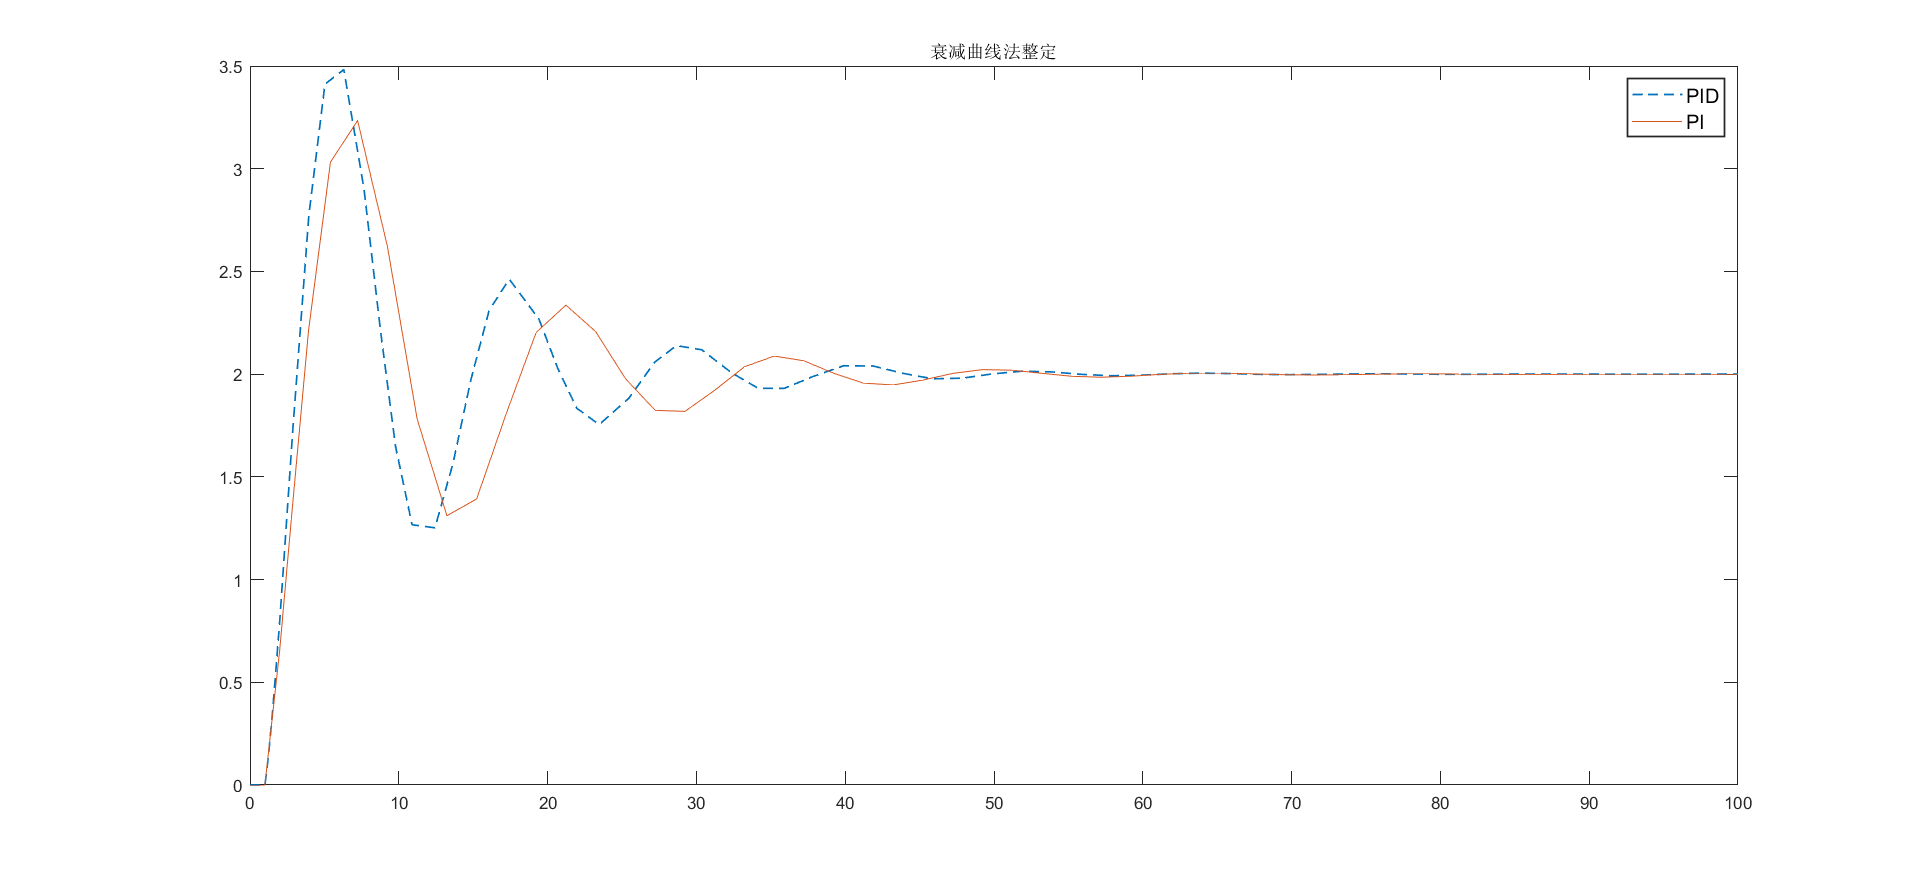
\includegraphics[width=12cm]{shuaijian.png}
	\caption{衰减曲线法整定结果} \label{fig4}
\end{figure}

图\ref{fig4}显示了采用衰减曲线法分别整定PID和PI控制作用参数后的系统响应曲线,其中PI的超调量为稳态值的62.5\%,稳态时间在65s左右,较之临界比例度法的整定过后系统的快速性和稳定性有所提升,这主要得益于采用衰减曲线法所计算出的比例系数$K_p$有所减小,积分时间$T_i$和$T_d$有所增大。因此,我们沿用此种改进思路,根据人工经验,继续适当的减小比例系数$K_p$,增大积分时间$T_i$和$T_d$,最终得出了改进后的整定结果($K_p=1.3$,  $\frac{1}{T_i}=0.2$,  $T_d=2.5$),如图\ref{fig5}.
\section{整定结果的分析和改进}

\begin{figure}[h]
	\small
	\centering
	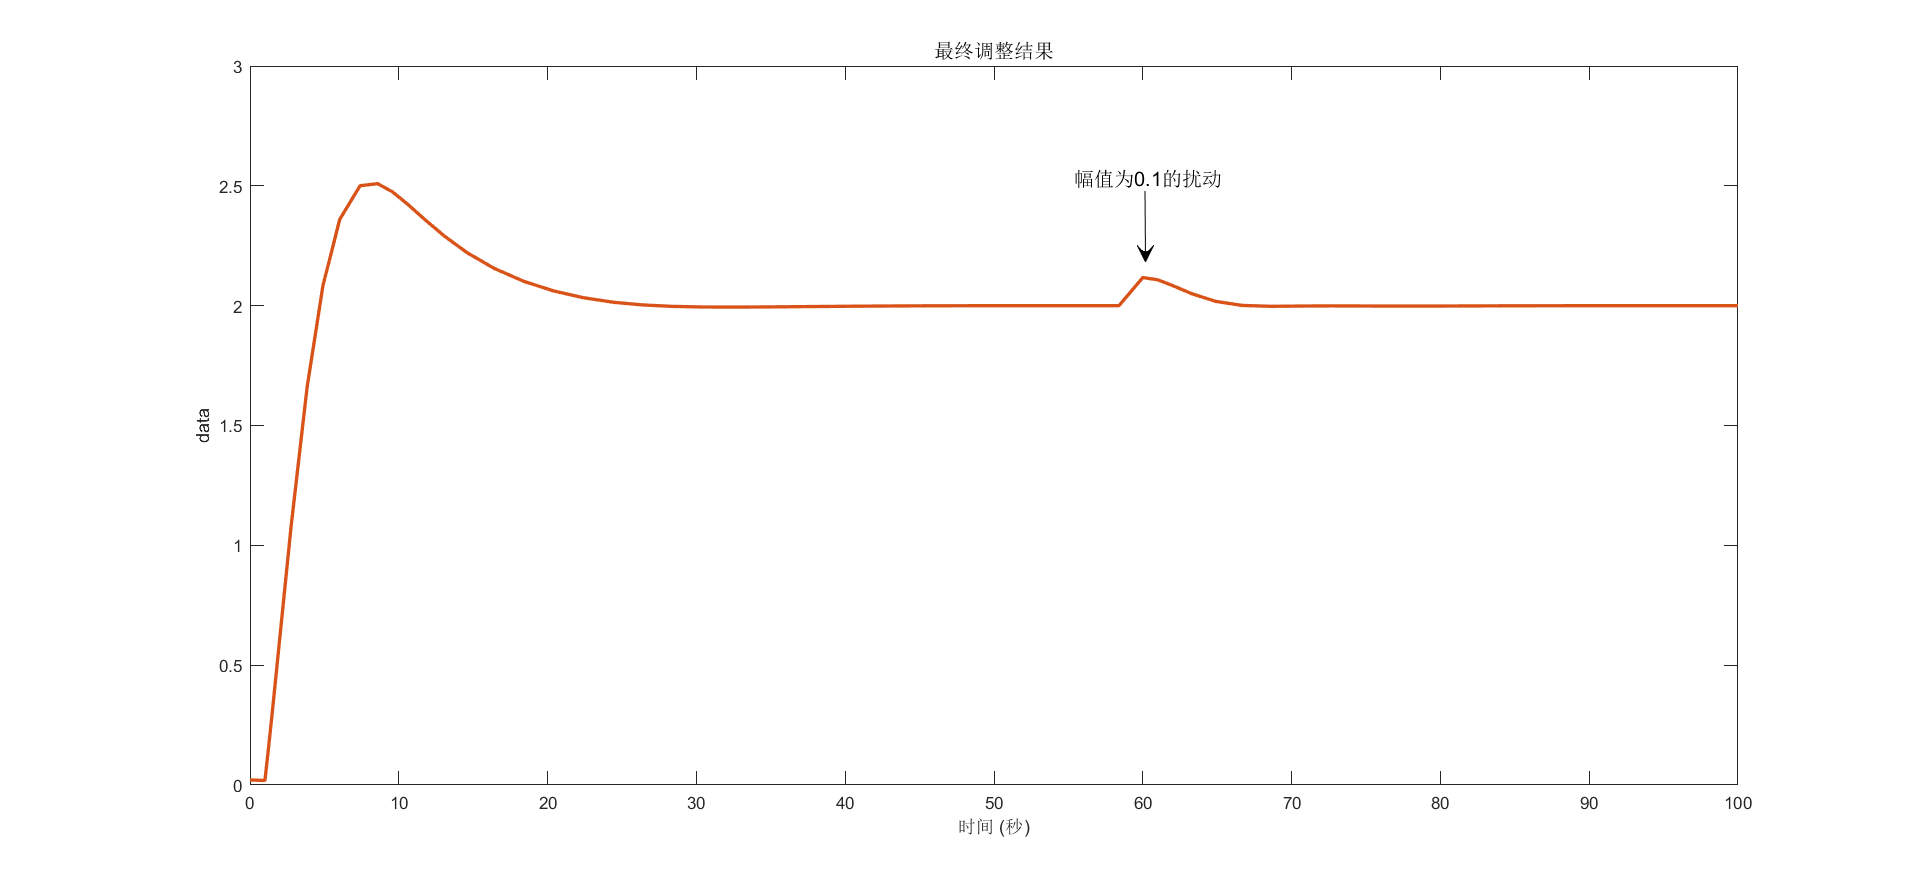
\includegraphics[width=12cm]{zuizhong.png}
	\caption{最终整定结果} \label{fig5}
\end{figure}
图\ref{fig5}显示:改进后的超调量为稳态值的50\%,并且系统进入稳态的时间在30s左右,其快速性和稳定性较之前结果有明显的提升。在60s时添加一个幅值为0.1的带限白噪声,系统在不到10s后又重新回到稳态,证明改进后的整定结果使系统具有较强的抗扰动性。本次实验结果表明,半经验法与人工经验最终修正的结合,是整定PID控制器参数的有效方法。

%\chapter{基于simulink的三容水箱液位控制仿真}

\chapter{基于simulink的三容水箱液位控制仿真}

\section{对于三容水箱系统的机理建模}
根据过程内在机理,应用物料和能量平衡及有关的化学、物理规律建立过程模型的方法是机理建模的方法,又称为过程动态学方法。其特点是建立的模型物理概念清晰、准确,可给出系统输入变量、输出变量、状态变量之间的关系。

\begin{figure}[h]
	\small
	\centering
	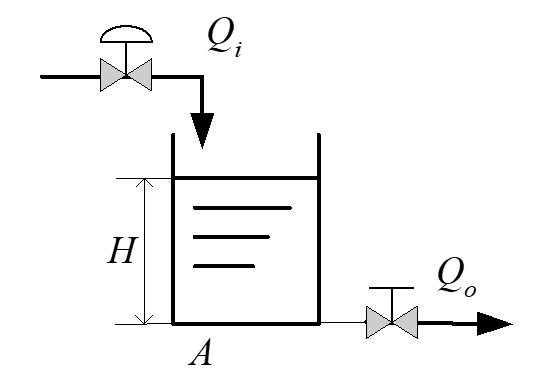
\includegraphics[width=5cm]{1water.png}
	\caption{单容水箱系统} \label{fig6}
\end{figure}


图\ref{fig6}是一个典型的单容水箱系统。根据物料守恒和流体运动学知识,我们可以建立单容水箱系统的数学模型:
\begin{equation}
\begin{cases}
A\frac{dH}{dT}=Q_i-Q_0\\
Q_0=k\sqrt{H}\\
\end{cases}
	\label{water1}
\end{equation}
其中:$Q_i,Q_0$分别表示阀门后的流体流量,$H$表示液位高度,$A$表示水箱的横截面积。我们可以据此建立三容水箱系统(图\ref{fig7})的数学模型:

$$
\left[ \begin{array}{c}
\dot{h}_1\\
\dot{h}_2\\
\dot{h}_3\\
\end{array} \right] =\frac{1}{A}\left[ \begin{array}{c}
-Q_{13}\\
Q_{32}-Q_{20}\\
Q_{13}-Q_{32}\\
\end{array} \right] +\frac{1}{A}\left[ \begin{array}{c}
\begin{matrix}
1&		0\\
\end{matrix}\\
\begin{matrix}
0&		1\\
\end{matrix}\\
\begin{matrix}
0&		0\\
\end{matrix}\\
\end{array} \right] \left[ \begin{array}{c}
Q_1\\
Q_2\\
\end{array} \right] +\left[ \begin{array}{c}
\eta _1\left( h,Q \right)\\
\eta _2\left( h,Q \right)\\
\eta _3\left( h,Q \right)\\
\end{array} \right] 
$$
\begin{equation}
\left[ \begin{array}{c}
y_1\\
y_1\\
\end{array} \right] =\left[ \begin{array}{c}
\begin{matrix}
1&		0&		0\\
\end{matrix}\\
\begin{matrix}
0&		1&		0\\
\end{matrix}\\
\end{array} \right] \left[ \begin{array}{c}
h_1\\
h_2\\
h_3\\
\end{array} \right] 
\label{water3.1}
\end{equation}
$$
Q_{13}=aZ_1S_psign\left( h_1-h_3 \right) \sqrt{2g\left| h_1-h_3 \right|}
$$
$$
Q_{32}=aZ_3S_psign\left( h_3-h_2 \right) \sqrt{2g\left| h_3-h_2 \right|}
$$
$$
Q_{20}=aZ_2S_p\sqrt{2gh_2}
$$



\begin{figure}[h]
	\small
	\centering
	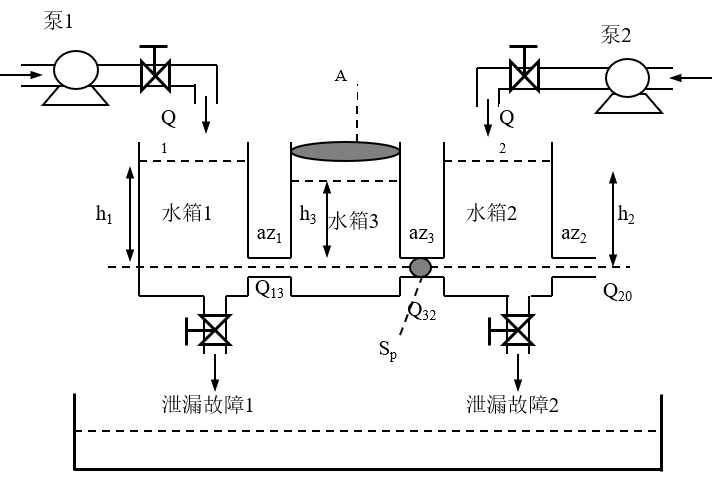
\includegraphics[width=12cm]{water3.png}
	\caption{三容水箱系统} \label{fig7}
\end{figure}
其中 $h_i$表示液位高度(cm)$i=1,2,3$,$Q_{13},Q_{32}$表示水箱之间的流速,$Q_1,Q_2$表示进水流速$\left( cm^3/s \right)$; A表示水箱的横截面积, $S_p$表示连接管的横截面积,$aZ_i$表示水
流系数,g表示重力加速度$\left( cm/s^2 \right)$.$sign\left(  \right) $表示符号函数。实验模型的技术参数数据:$A=154cm^2,S_p=0.5cm^2,aZ_1=0.45,aZ_2=0.61,aZ_3=0.46,Q_{\text{1}\max}=Q_{\text{2}\max}=100cm^3/s,h_{\max}=62cm$,$=980\left( cm/s^2 \right) $
\section{基于simulink的三容水箱液位控制仿真}

\begin{figure}[h]
	\small
	\centering
	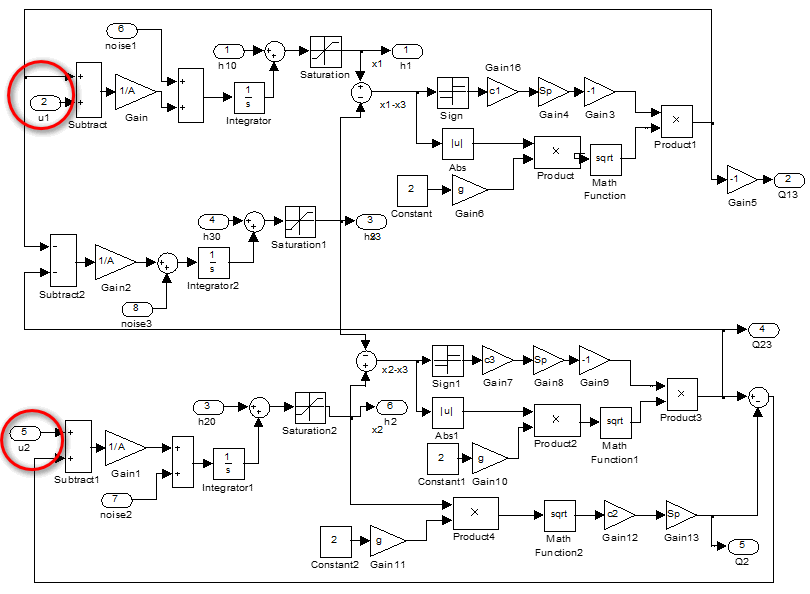
\includegraphics[width=10.5cm]{bcm.png}
	\caption{参考文献中的三容水箱系统simulink模型搭建} \label{fig8}
\end{figure}

图\ref{fig8}是参考文献中对于三水箱液位系统的simulink搭建,在阅读本图时,我们对PID模块(控制器)应该放置的位置产生了疑惑:图\ref{fig8}中用两个红色圆圈标记的两路信号分别是$u_1$(即图\ref{fig7}中的$Q_1$,量纲为$cm^3/s$)与$h_1$(量纲为$cm$)之差,$u_2$(即图\ref{fig7}中的$Q_2$,量纲为$cm^3/s$)与$h_2$(量纲为$cm$)之差.我们对于两个量纲不同的物理量作差的画法感到有些困惑,并且本系统需要实现的要求是:用户设定一号和二号水箱的设定值,通过PID控制器控制一,二号水箱的阀门开度,进而使系统最终和用户的设定值无静差。在参考文献的画法中,PID模块究竟应该放置在什么位置?控制器的输出与流量又具有怎样的关系?这是我们需要解决的关键性问题。


经过思考后,我们重新审视了PID控制器的核心:即控制器的输出一定是偏差信号(在本系统中指用户对于一,二号水箱的期望设定值与实际液位值的差),所以PID模块一定要放在偏差信号后面,至于PID模块的输出,我们可以完全理解为是一个电信号,这个电信号包含了PID模块校正的控制信息,至于执行器(阀门)是如何解读这一信号的,我们觉得对于仿真结果完全没有任何影响。所以我们以参考文献的画法为基础,对红色标记的区域做了微小改动。如图\ref{fig9}.
\newline 
\begin{figure}[h]
	\small
	\centering
	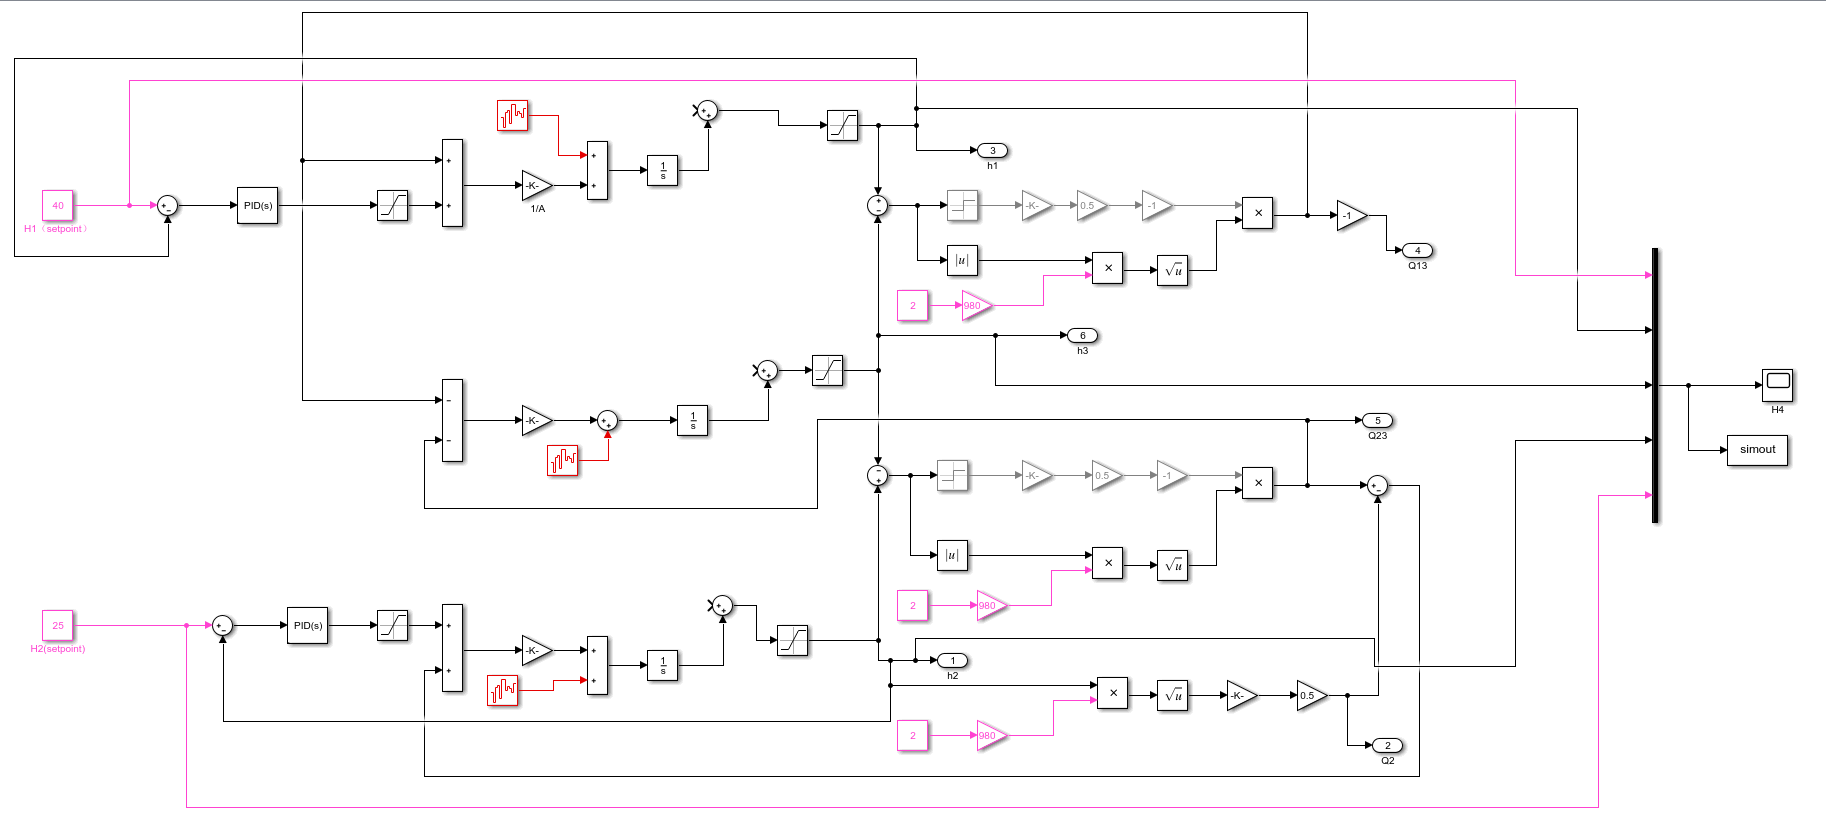
\includegraphics[width=16cm]{3watersim.png}
	\caption{三容水箱系统simulink模型搭建} \label{fig9}
\end{figure}

在未加扰动的情况下,设定$H_1(setpoint)=40(cm),H_2(setpoint)=25(cm)$,$H_1,H_2,H_3$三个水箱的初始液位是0.利用半经验法和人工经验最终修正调整图\ref{fig9}中两个PID的参数,我们最终得到一号水箱PID的参数为:比例系数$K_p=20$,$\frac{1}{T_i}=0.44$,$T_d=20$,二号随想PID的参数为:比例系数$K_p=20$,$\frac{1}{T_i}=0.55$,$T_d=20$.系统响应如图\ref{fig10}.

\begin{figure}[h]
	\small
	\centering
	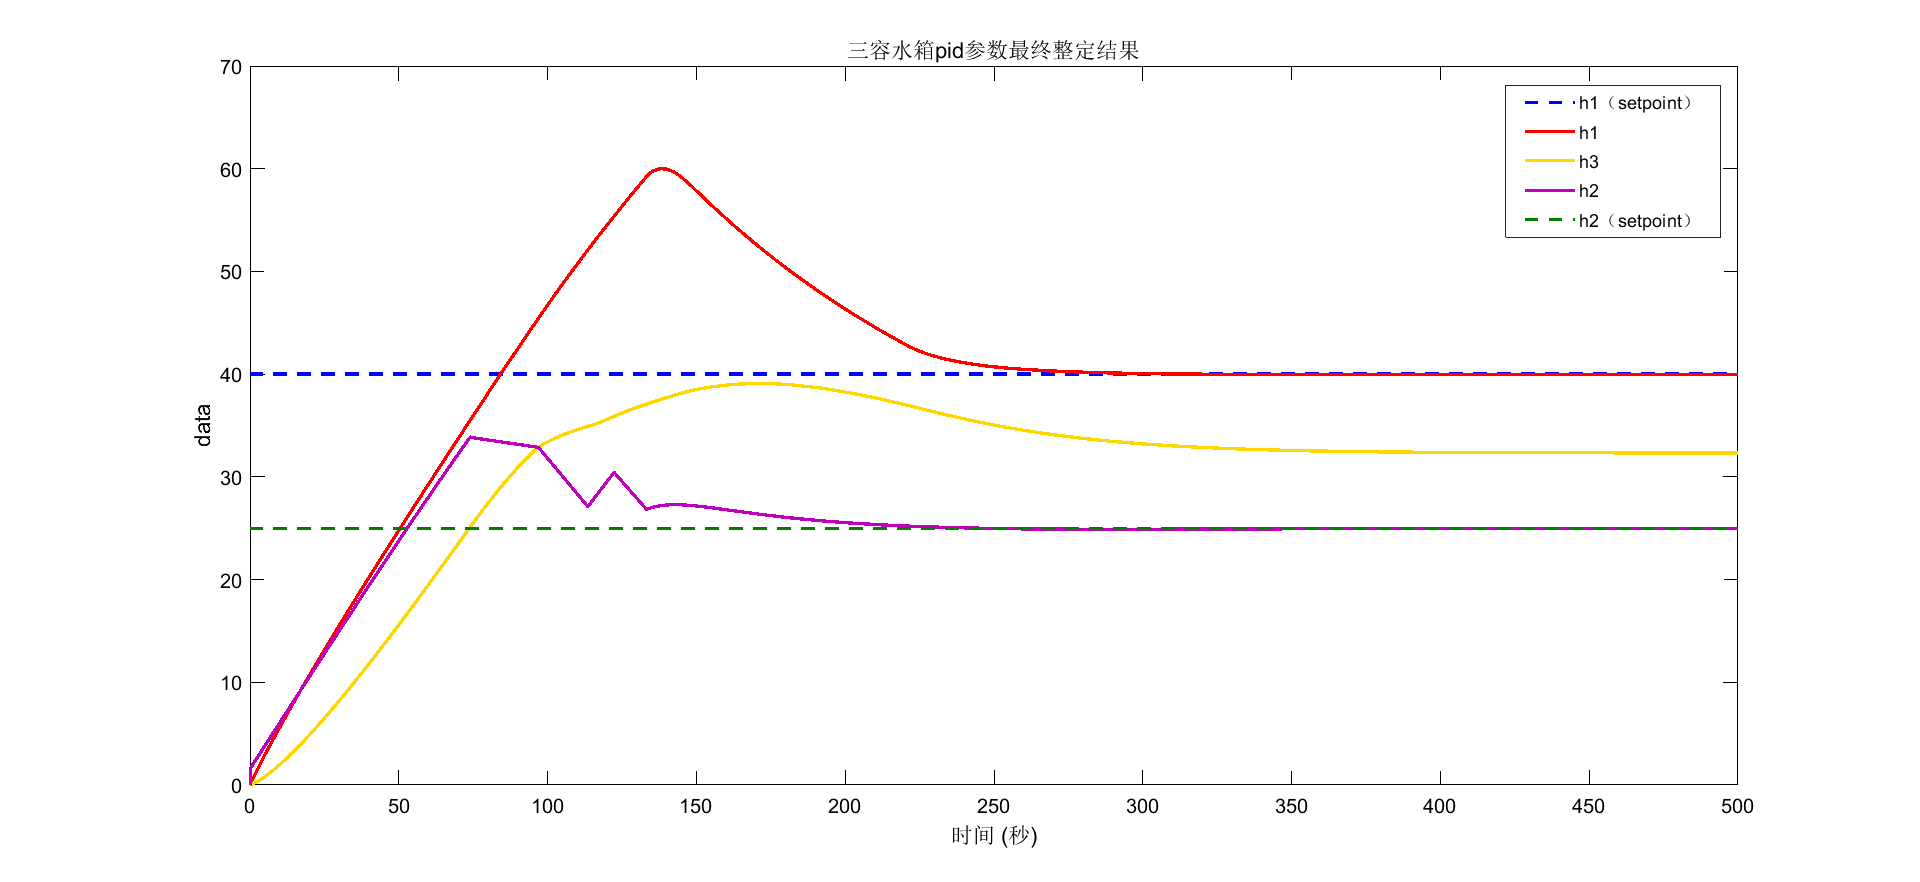
\includegraphics[width=16cm]{3waterzuizhong.png}
	\caption{未加噪声的三容水箱系统最终整定} \label{fig10}
\end{figure}

三水箱系统是一个大时滞,大惯性的系统。从图中可以明显看出:一号水箱具有50\%的超调量,在250s左右完全消除稳态误差;二号水箱具有40\%的超调量,在200s左右基本消除稳态误差,对于工业级系统而言,本次整定的效果较好。为了测试PID校正后系统的抗干扰性,我们为每个水箱都添加了不同幅度的带限白噪声(采样时间为0.5s):一号水箱带限白噪声幅值=0.35$cm$,二号水箱带限白噪声幅值=0.25$cm$,三号水箱带限白噪声幅值=0.65$cm$.系统响应结果如图\ref{fig11}.

\begin{figure}[h]
	\small
	\centering
	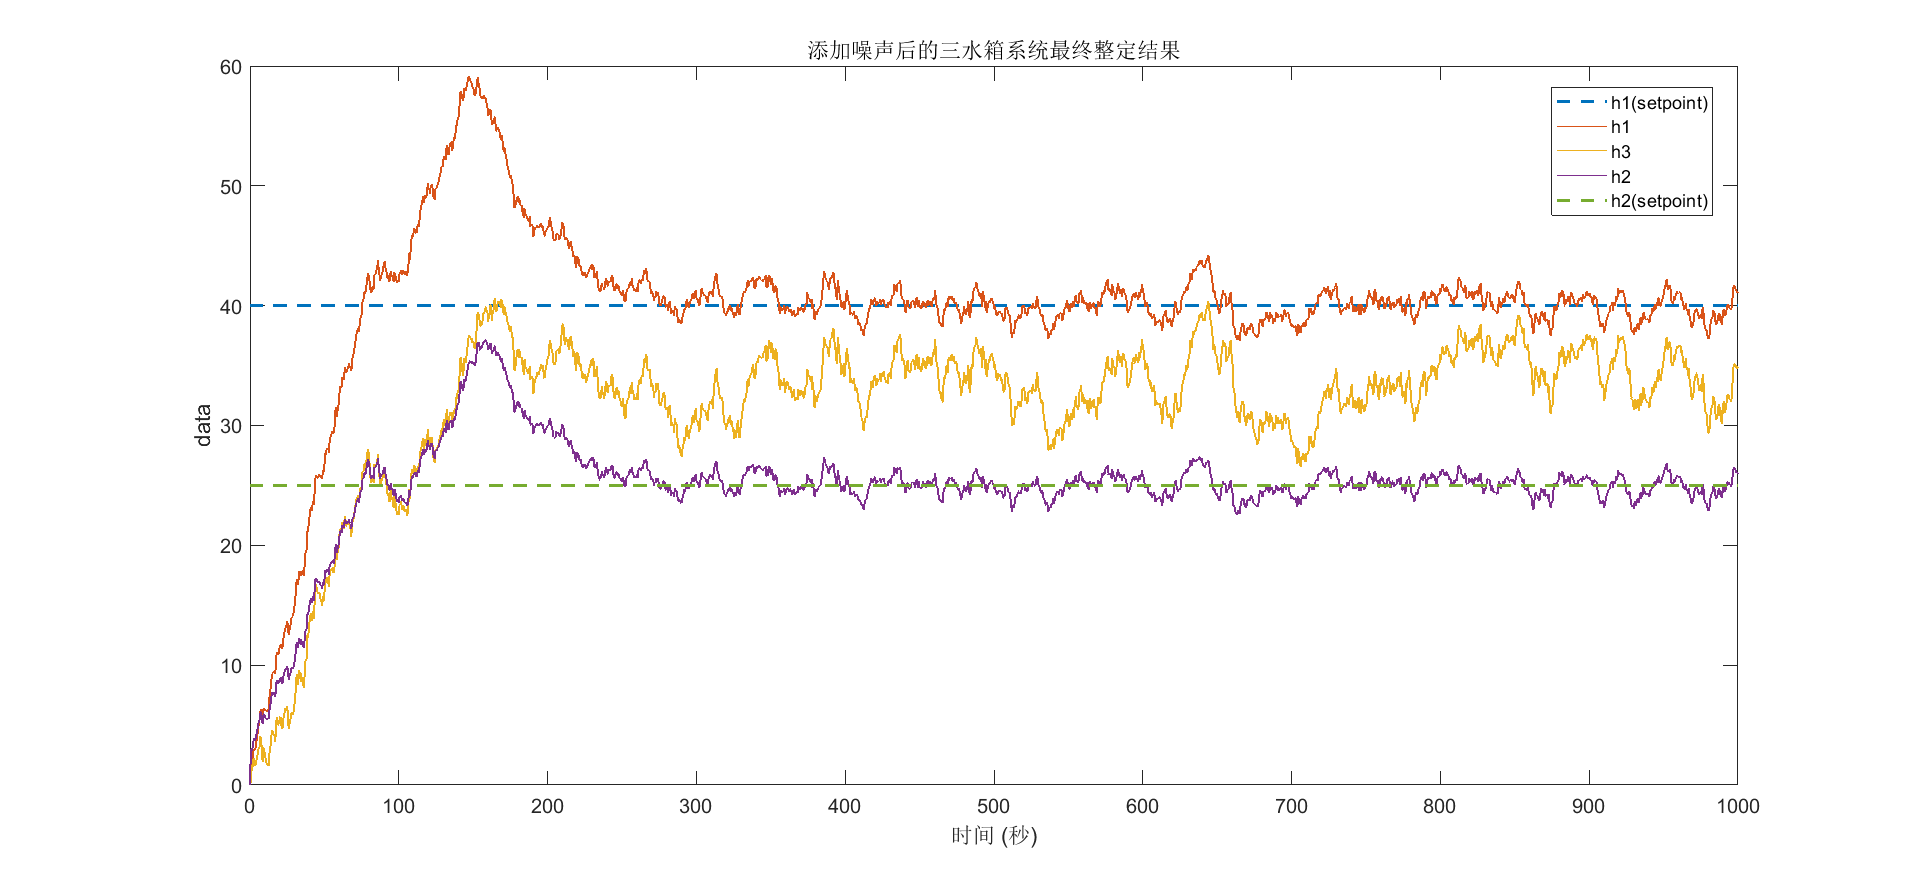
\includegraphics[width=16cm]{3waterzaosheng.png}
	\caption{添加噪声后的三容水箱系统最终整定} \label{fig11}
\end{figure}



% Table generated by Excel2LaTeX from sheet 'Sheet1'
% \begin{table}[htbp]
% 	\centering
% 	\caption{控制度法整定数字控制器参数}
% 	\setlength{\leftskip}{-50pt}
% 	\begin{tabular}{ccccccccccccc}
% 		\toprule
% 		\multicolumn{3}{c}{控制度} & \multicolumn{2}{c}{控制作用} & \multicolumn{2}{c}{$T_s$} & \multicolumn{2}{c}{$K_c$} & \multicolumn{2}{c}{$T_i$} & \multicolumn{2}{c}{$T_d$} \\
% 		\midrule
% 		\midrule
% 		\multicolumn{3}{c}{1.05} & \multicolumn{2}{c}{PI // PID} & \multicolumn{2}{c}{0.03$T_k$ // 0.014$T_k$} & \multicolumn{2}{c}{0.53$K_{ck}$ // 0.63$K_{ck}$} & \multicolumn{2}{c}{0.85$T_k$ // 0.49$T_k$} & \multicolumn{2}{c}{-// 0.14$T_k$} \\
% 		\multicolumn{3}{c}{1.2} & \multicolumn{2}{c}{PI // PID} & \multicolumn{2}{c}{0.05$T_k$ // 0.043$T_k$} & \multicolumn{2}{c}{0.49$K_{ck}$ // 0.47$K_{ck}$} & \multicolumn{2}{c}{0.91$T_k$ // 0.47$T_k$} & \multicolumn{2}{c}{-// 0.16$T_k$} \\
% 		\multicolumn{3}{c}{1.5} & \multicolumn{2}{c}{PI // PID} & \multicolumn{2}{c}{0.14$T_k$ // 0.09$T_k$} & \multicolumn{2}{c}{0.42$K_{ck}$ // 0.24$K_{ck}$} & \multicolumn{2}{c}{0.99$T_k$ // 0.43$T_k$} & \multicolumn{2}{c}{-// 0.20$T_k$} \\
% 		\multicolumn{3}{c}{2} & \multicolumn{2}{c}{PI // PID} & \multicolumn{2}{c}{0.22$T_k$ // 0.16$T_k$} & \multicolumn{2}{c}{0.36$K_{ck}$ // 0.27$K_{ck}$} & \multicolumn{2}{c}{1.05$T_k$ // 0.40$T_k$} & \multicolumn{2}{c}{-// 0.22$T_k$} \\
% 		\multicolumn{3}{c}{模拟控制器} & \multicolumn{2}{c}{PI // PID} & \multicolumn{2}{c}{} & \multicolumn{2}{c}{0.57$K_{ck}$ // 0.70$K_{ck}$} & \multicolumn{2}{c}{0.83$T_k$ // 0.50$T_k$} & \multicolumn{2}{c}{-// 0.13$T_k$} \\
% 		\multicolumn{3}{c}{Ziegler和Nichols建议值} & \multicolumn{2}{c}{PI // PID} & \multicolumn{2}{c}{} & \multicolumn{2}{c}{0.45$K_{ck}$ // 0.60$K_{ck}$} & \multicolumn{2}{c}{0.83$T_k$ // 0.50$T_k$} & \multicolumn{2}{c}{-// 0.125$T_k$} \\
% 		\bottomrule
% 	\end{tabular}%
% 	\label{tab3}%
% \end{table}%



% Table generated by Excel2LaTeX from sheet 'Sheet1'
% \begin{table}[htbp]
% 	\centering
% 	\caption{Add caption}
% 	\begin{tabular}{cccccccc}
% 		\toprule
% 		\multicolumn{2}{c}{控制作用} & \multicolumn{2}{c}{kc} & \multicolumn{2}{c}{ti} & \multicolumn{2}{c}{td} \\
% 		\midrule
% 		\midrule
% 		\multicolumn{2}{c}{\multirow{2}[1]{*}{P}} & \multicolumn{2}{c}{\multirow{2}[1]{*}{$\frac{T}{K_0\tau}\left( 1+\frac{\tau}{3T} \right)$ }} & \multicolumn{2}{c}{\multirow{2}[1]{*}{}} & \multicolumn{2}{c}{\multirow{2}[1]{*}{}} \\
% 		\multicolumn{2}{c}{} & \multicolumn{2}{c}{} & \multicolumn{2}{c}{} & \multicolumn{2}{c}{} \\
% 		\multicolumn{2}{c}{\multirow{2}[0]{*}{PI}} & \multicolumn{2}{c}{\multirow{2}[0]{*}{$\frac{T}{K_0\tau}\left( 0.9+\frac{\tau}{12T} \right) $}} & \multicolumn{2}{c}{\multirow{2}[0]{*}{$\tau \left( \frac{30+3\tau /T}{9+20\tau /T} \right)$}} & \multicolumn{2}{c}{\multirow{2}[0]{*}{}} \\
% 		\multicolumn{2}{c}{} & \multicolumn{2}{c}{} & \multicolumn{2}{c}{} & \multicolumn{2}{c}{} \\
% 		\multicolumn{2}{c}{\multirow{2}[1]{*}{PID}} & \multicolumn{2}{c}{\multirow{2}[1]{*}{$\frac{T}{K_0\tau}\left( \frac{4}{3}+\frac{\tau}{4T} \right)$}} & \multicolumn{2}{c}{\multirow{2}[1]{*}{$\tau \left( \frac{32+6\tau /T}{13+8\tau /T} \right)$ }} & \multicolumn{2}{c}{\multirow{2}[1]{*}{$\tau \left( \frac{4}{11+2\tau /T} \right)$ }} \\
% 		\multicolumn{2}{c}{} & \multicolumn{2}{c}{} & \multicolumn{2}{c}{} & \multicolumn{2}{c}{} \\
% 		\bottomrule
% 	\end{tabular}%
% 	\label{tab:addlabel}%
% \end{table}%












%%%=== 参考文献 ========%%%
\cleardoublepage\phantomsection
\addcontentsline{toc}{chapter}{参考文献}
\begin{thebibliography}{000}\zihao{5}

  \bibitem{r1} 作者, 文章题目, 期刊名, 年份(期数): 起止页码

  \bibitem{r2} 作者, 书名, 年份, 版次, 出版地: 出版单位, 起止页码

  \bibitem{r3} 邓建松等, 《\LaTeXe~科技排版指南》, 科学出版社

  \bibitem{r4} 吴凌云, 《CTeX~FAQ (常见问题集)》, \textit{Version~0.4}, June 21, 2004

  \bibitem{r5} Herbert Vo\ss, Mathmode, \url{http://www.tex.ac.uk/ctan/info/math/voss/mathmode/Mathmode.pdf}.

\end{thebibliography}



\backmatter
% !Mode:: "TeX:UTF-8"

%%% 此部分内容:  (1) 致谢  (2) 武汉大学学位论文使用授权协议书(无需改动)

%%%%%%%%%%%%%%%%%%%%%%%
%%% --------------- 致谢 ------------- - %%%
%%%%%%%%%%%%%%%%%%%%%%%
\acknowledgement


感谢你, 感谢他和她, 感谢大家.







%%%%%---武汉大学学位论文使用授权协议书---%%%%%%%%%%%%
%%%%%%%%%%%%%%%%%%%%%%%%%%%%%%%%%%%
%%%%%%%%%%%%%%%%%%%%%%%%%%%%%%%%%%%
\cleardoublepage
\newpage\vspace*{20pt}
\begin{center}{\zihao{-2}\heiti 武汉大学学位论文使用授权协议书}\end{center}
\par\vspace*{30pt}

本学位论文作者愿意遵守武汉大学关于保存、使用学位论文的管理办法及规定,
即:学校有权保存学位论文的印刷本和电子版, 并提供文献检索与阅览服务;
学校可以采用影印、缩印、数字化或其它复制手段保存论文;
在以教学与科研服务为目的前提下, 学校可以在校园网内公布部分及全部内容.
\begin{enumerate}[1、]
  \item  在本论文提交当年, 同意在校园网内以及中国高等教育文献保障系
           统(CALIS)高校学位论文系统提供查询及前十六页浏览服务.
  \item  在本论文提交~$\Box$~当年/~$\Box$~一年/~$\Box$~两年
            /~$\Box$~三年/~$\Box$~五年以后, 同意在校园网内允许读者
            在线浏览并下载全文, 学校可以为存在馆际合作关系的兄弟高校用
            户提供文献传递服务和交换服务.(保密论文解密后遵守此规定)
\end{enumerate}

\vskip 15mm

论文作者(签名):\raisebox{-1ex}{\underline{\makebox[5cm][c]{}}}
\vskip2em
				          				
学\qquad\qquad\quad 号:\raisebox{-1ex}{\underline{\makebox[5cm][c]{}}}
\vskip2em	
					
学\qquad\qquad\quad 院:\raisebox{-1ex}{\underline{\makebox[5cm][c]{}}}					

\vskip  2cm
\begin{flushright}
 日期:\hskip2cm 年\hskip1.2cm 月\hskip1.2cm 日
\end{flushright}

%%%%%%%%%%%%%%%%%%%%%%%%%%%%%%%%%%%%%%%
%%%%%%%--判断是否需要空白页-----------------------------
  \iflib
  \else
  \newpage
  \cleardoublepage
  \fi
%%%%%%%-------------------------------------------------







 %%%致谢, 武汉大学学位论文使用授权协议书.
\cleardoublepage
\end{document}



